%%%%%%%%%%%%%%%%%%%%%%%%%%%%%%%%%%%%%%%%%
% Stylish Article
% LaTeX Template
% Version 2.2 (2020-10-22)
%
% This template has been downloaded from:
% http://www.LaTeXTemplates.com
%
% Original author:
% Mathias Legrand (legrand.mathias@gmail.com)
% With extensive modifications by:
% Vel (vel@latextemplates.com)
%
% License:
% CC BY-NC-SA 3.0 (http://creativecommons.org/licenses/by-nc-sa/3.0/)
%
%%%%%%%%%%%%%%%%%%%%%%%%%%%%%%%%%%%%%%%%%

%----------------------------------------------------------------------------------------
%	PACKAGES AND OTHER DOCUMENT CONFIGURATIONS
%----------------------------------------------------------------------------------------

\documentclass[fleqn,10pt]{SelfArx} % Document font size and equations flushed left

\usepackage[english]{babel} % Specify a different language here - english by default

\usepackage{lipsum} % Required to insert dummy text. To be removed otherwise
\usepackage{listings}
\usepackage{tcolorbox}
\usepackage{graphicx}
\usepackage[ruled,linesnumbered]{algorithm2e}
\usepackage[noend]{algpseudocode}
\usepackage{algorithm2e}

%----------------------------------------------------------------------------------------
%	COLUMNS
%----------------------------------------------------------------------------------------

\setlength{\columnsep}{0.55cm} % Distance between the two columns of text
\setlength{\fboxrule}{0.75pt} % Width of the border around the abstract

%----------------------------------------------------------------------------------------
%	COLORS
%----------------------------------------------------------------------------------------

\definecolor{color1}{RGB}{0,0,90} % Color of the article title and sections
\definecolor{color2}{RGB}{0,20,20} % Color of the boxes behind the abstract and headings

%----------------------------------------------------------------------------------------
%	HYPERLINKS
%----------------------------------------------------------------------------------------

\usepackage{hyperref} % Required for hyperlinks

\hypersetup{
	hidelinks,
	colorlinks,
	breaklinks=true,
	urlcolor=color2,
	citecolor=color1,
	linkcolor=color1,
	bookmarksopen=false,
	pdftitle={Title},
	pdfauthor={Author},
}

%----------------------------------------------------------------------------------------
%	ARTICLE INFORMATION
%----------------------------------------------------------------------------------------

\PaperTitle{GCC - A Lightweight, Accesible, and User-Friendly Workflow Execution Service}

\Authors{Nathan Loria\textsuperscript{1}*}
\affiliation{\textsuperscript{1}\textit{Department of Computer Science, Allegheny College, Meadville, PA}}
\affiliation{*\textbf{Corresponding author}: lorian@allegheny.edu}

\Keywords{Workflow -- Cloud Computing -- Task Scheduling}
\newcommand{\keywordname}{Keywords}

%----------------------------------------------------------------------------------------
%	ABSTRACT
%----------------------------------------------------------------------------------------

\Abstract{A workflow is a cluster of nodes that work together to accomplish an end goal. When executing a workflow, especially one associated with big data, there is often a massive amount of data and time overhead to work around. Because of this, there is a large need for efficient and easy to use software which allows for the execution of workflows on obscure computing resources, which removes the need for massive infrastructure investments by the party that is executing a workflow. Additionally, the demand for efficient task scheduling solutions is ever-increasing. All of these are issues which can be tackled with the proper implementation of a cloud computing system. This cloud computing approach combined with efficient task scheduling is the focus of our project: Gator Computational Cloud (GCC). GCC is a lightweight web framework that utilizes a generic task scheduling algorithm to schedule jobs in a cloud environment. This framework intelligently manages dependencies, and takes a multi-threaded execution approach in order to increase efficiency. In order to execute nodes, GCC takes advantage of the Amazon AWS Java API to provision nodes. Once provisioned, the tool completes the execution and transfers any dependencies to their corresponding VM. The goal of the project is to provide a light weight and user friendly environment for workflow execution, while also ensuring a powerful and efficient backend which completes a users workflow with ease. In order to achieve this, some preliminary experimentation has taken place to ensure the effectiveness of the tool.}

%----------------------------------------------------------------------------------------

\begin{document}

\maketitle % Output the title and abstract box

\tableofcontents % Output the contents section

\thispagestyle{empty} % Removes page numbering from the first page

%----------------------------------------------------------------------------------------
%	ARTICLE CONTENTS
%----------------------------------------------------------------------------------------

\section{Introduction}
\label{sec:introduction}

\begin{figure*}[t!]
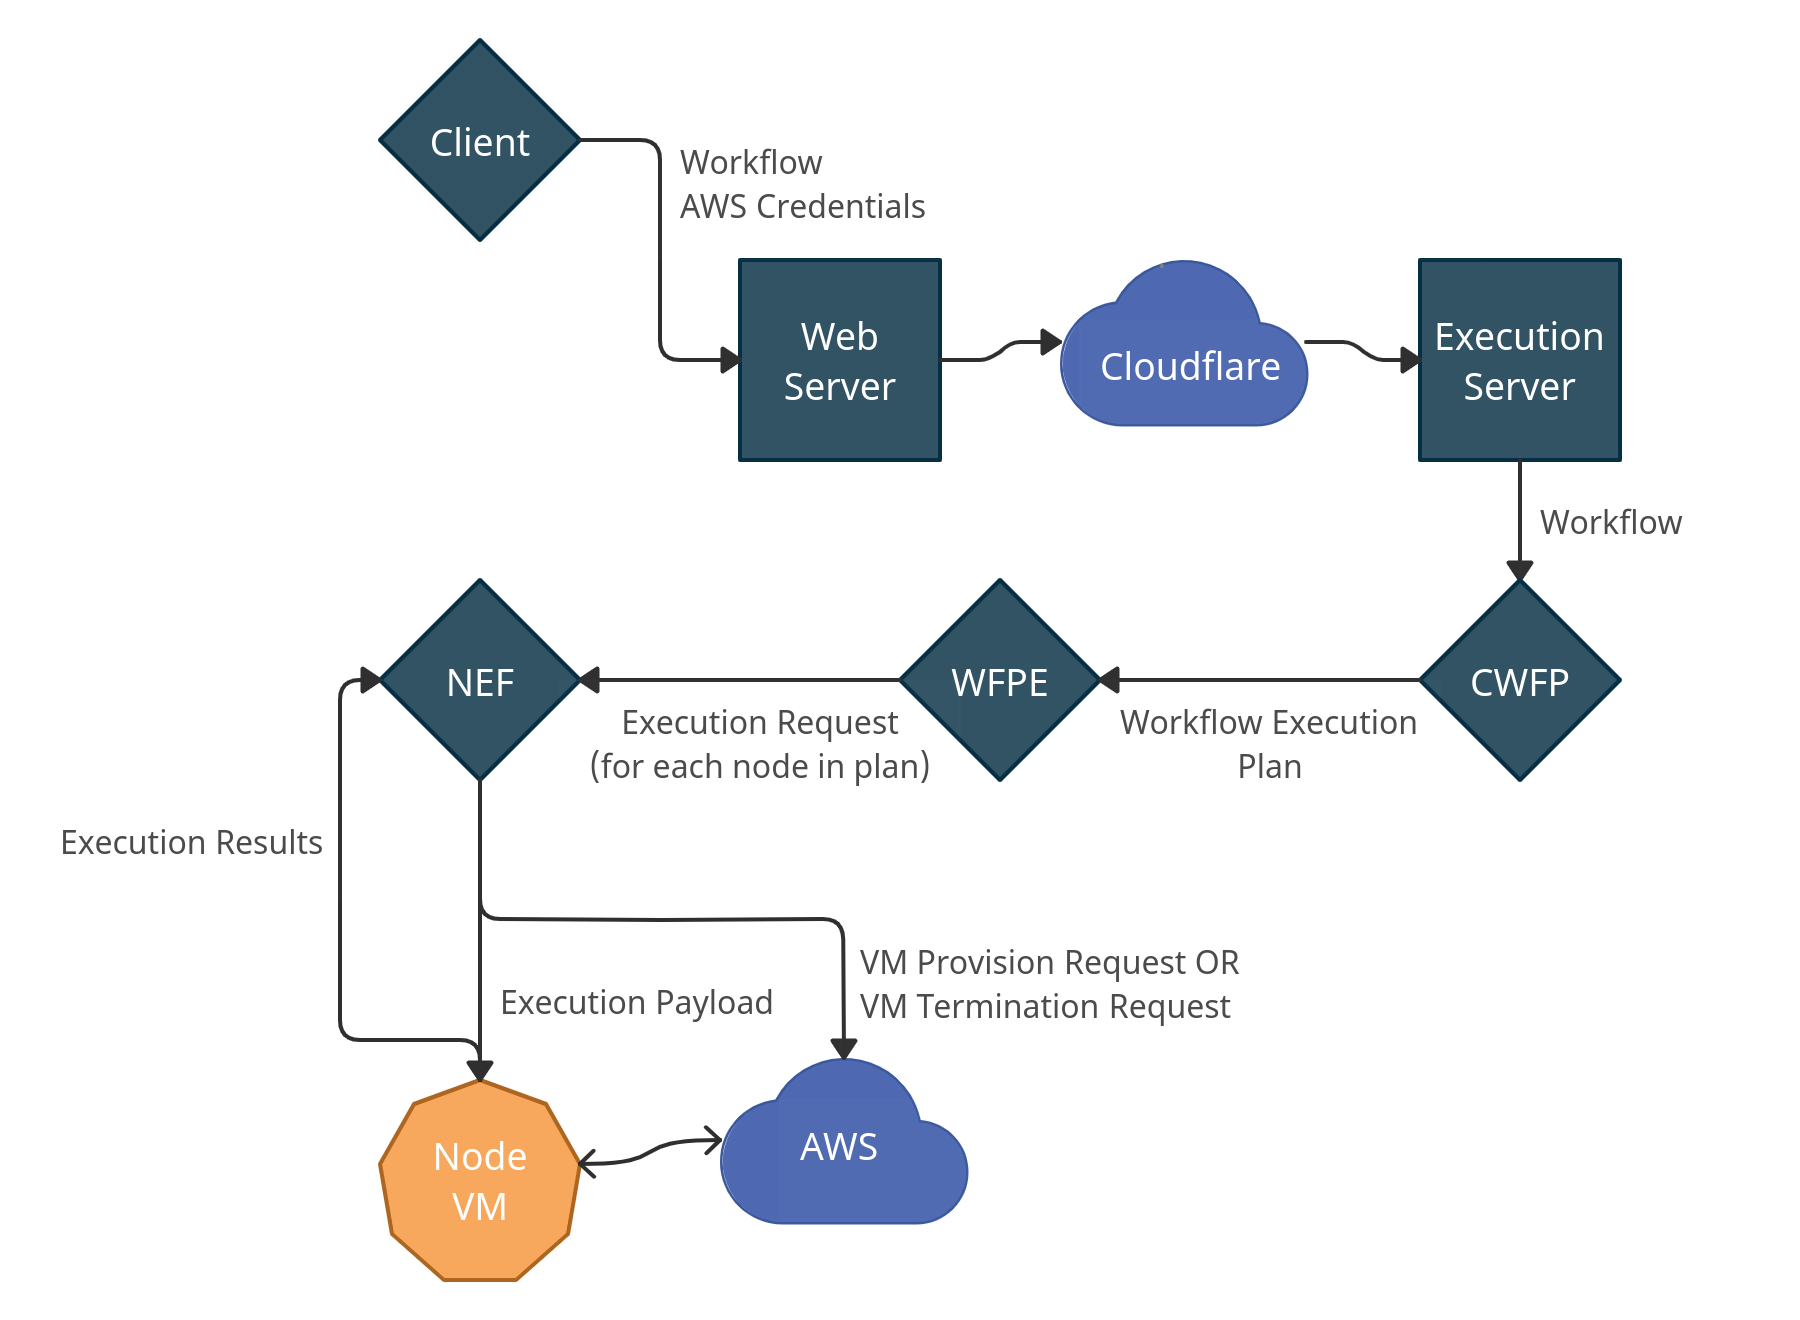
\includegraphics[width=\textwidth]{Figures/gcc_total_workflow.png}
\caption{An example architecture of GCC}
\label{fig:gccworkflow}
\end{figure*}

As time passes, the world is being driven faster and faster towards a more technocentric and data-centric future. Because of this, there is an ever-increasing need for more efficient, powerful, and usable frameworks for big data management and processing. This phenomenon is known as datafication. It not only raises issues of technical capacity, but also of social equity \cite{mejias2019datafication}. Needless to say, it is an issue that is, and will remain, very prominent in almost all aspects of life. With such increase in the overall amount of data that is available in today's world, it can be challenging for people with not a lot of resources or experience with cloud computing to process this data. Even individuals who may have the knowledge to do so, using computational strategies, are often met with the issue of available infrastructure. Computations on large data are almost always extremely resource intensive. This can make it hard for those who do not have access to powerful computing systems to do what they need to do in a reasonable amount of time. This is where the issue of cloud computing and, more specifically, workflow scheduling comes into play.

Already, there can be observed a large shift in focus from local software systems such as older versions of Microsoft's Office (Excel, Access, Word) to cloud-based software such as Google's G-Suite (Docs, Slides, Sheets) for everyday users. This phenomenon is known as software as a service (hereafter referred to as SaaS) and it is becoming very popular in both business and everyday applications. In order to compete with Google, Microsoft released Office 365 which is a cloud-based version of their original suite. This shift was inevitable and now smaller \cite{kim2017analysis} and larger corporations are beginning to convert from previous versions of Office to the newer Office 365 \cite{skendzic2012microsoft} in order to reduce the need for more powerful computational devices. Both Google and Microsoft also offer their own versions of heterogeneous storage systems (Google Drive, Microsoft OneDrive) which are an example of infrastructure as a service (hereafter referred to as IaaS). These two combined principles (SaaS and IaaS) offer a glimpse into the future of computing.

In this paper, we propose a new web-based workflow execution platform called GCC (Gator Computational Cloud) which is used to execute computational workflows in a cloud environment. For the scope of this project, Java computations are the intended use case. GCC consists of 4 main components: an accessible and easy to use frontend UI (AUI), a workflow planner (CWFP), a node-based execution framework (NEF), and a plan executor (WFPE). Each of these components work together to provide a user with an extremely powerful tool without the need to worry about infrastructure investments or local computer resources. It is for this reason that GCC is an example of a framework that combines both SaaS and IaaS principles. It's web-based frontend combined with a powerful backend where data and nodes can be stored make it a great option for users who may not have the ability to execute their workflows on infrastructure of their own, or pay for the expensive software licenses associated with other localized workflow execution software. The architecture of this program is provided in \ref{fig:gccworkflow}.

This paper is structured as follows. Section \hyperref[sec:methods]{2} introduces the general structure of the GCC framework and introduces the design of the AUI, as well as the CWFP, WFPE, and NEF algorithms using examples. The preliminary experimental results are discussed in section \hyperref[sec:expresults]{3}. In section \hyperref[sec:relatedwork]{4}, the work related to that done in this project is discussed. Finally, section \hyperref[sec:conclusion]{5} concludes the paper and discusses future directions and possible areas of improvement to explore.

%------------------------------------------------

\section{Methods}
\label{sec:methods}

As previously mentioned, GCC consists of 4 main components: AUI, CWFP, NEF, and WFPE. The first component, AUI (accessible user interface) is a pivotal piece to fostering an effective user friendly environment. The AUI is the source that hosts GCC's web interface. It does so by utilizing the Django Python library and Apache 2 to serve static files. The next component, CWFP (comprehensive workflow planner) is an algorithm that takes in an XML file that is uploaded by a user and translates it into a directed acyclic graph which is used in later execution steps. This algorithm breaks the workflow into levels which allows the WFPE algorithm to do its job properly. The WFPE (workflow plan executor) component is an algorithm that takes in a workflow plan from the CWFP and calls each node's NEF which allows it to run. This is the backbone of the function of the program. The NEF (node execution framework) component is what actually calls the steps to execute a node. This includes the provisioning of instances, the uploading, downloading, and transferring of resources, and the execution of a payload on a node.

\subsection{AUI}

As mentioned before, the AUI component of the project is the component that provides a user with an efficient and accessible interface for operating the GCC service. The implementation is simple yet pivotal to the performance of GCC as a whole. Below are the three aspects of the AUI that enable it to do it's job effectively and efficiently.

\subsubsection{Content}

The AUI can be seen by travelling to gatorcompcloud.com on any current web browser that is actively supported and maintained. It consists of a login, signup, about us, and welcome page as well as three menu options entitled "Import a Workflow", "Execute a Workflow", and "AWS Credentials" respectively when on the welcome page. Upon a visit to the website, the user is prompted to input their GCC credentials. If a user does not already have an account with GCC, they are directed to the signup page where they can create an account for the tool. This page contains a lot of validation to ensure that a user provided valid information as well as a unique username. Once a user has created an account with valid credentials, they can then login using the login page. Upon verification of a user's credentials, the login page redirects to the welcome page for a user which gives a brief overview of how the tool works and what it's designed to do. This is the same page that displays the three menu options listed above, and each menu can be accessed at the user's will.

Located on the "Import a Workflow" page is a form which allows the user to upload their workflow source code. For the purpose of this project, a workflow is structured as a specification file (in XML format) and a collection of ZIP archives containing the payload that is to be executed for each node in a workflow. Once these items are uploaded, the tool creates an object for each of them and stores that object in the websites database. In GCC, each ZIP archive correlates to one node in a workflow. The structure of a workflow specification file can be observed in \ref{fig:xmlspec}. Additionally, the structure of a node archive file can be observed in \ref{fig:nodestructure}. In \ref{fig:xmlspec}, directories are surrounded by vertical lines in order to signify that they are a directory. Any item that is not surrounded by these lines is a file. Please note that for any nodes which require execution-dependent data when they are uploaded, this data should be placed in the "data/in" folder prior to uploading. This figure is an example of a valid node structure starting from the base archive file (EX\_NODE.zip) and travelling all the way to the nodes source code (EX\_CODE.java). The two scripts (build.sh and run.sh) are used to formalize the execution process and ensure that execution errors do not occur from GCC's side. In \ref{fig:nodestructure}, the workflow being exemplified is one that contains 4 nodes: n1, n2, n3, and n4. For each node, a list of dependencies is listed. In the case of this example, this workflow would create a diamond shaped when represented graphically as n2 and n3 directly rely on n1, and n4 directly relies on n2 and n3 in order for the execution to function properly. Please note that for each specification file that is uploaded, the name of the workflow object created in the GCC framework will be the name of the XML specification file with the ".xml" extension stripped. The same goes for node object names, except the ".zip" extension is stripped.

\begin{figure}[t]
\centering
\begin{tcolorbox}[boxrule=0.5pt,colback=cyan!15!white]
\begin{lstlisting}[basicstyle=\footnotesize, frame=lines]
<?xml version="1.0"?>
<workflow>
    <task>
        <id>n1</id>
        <deps></deps>
    </task>
    <task>
        <id>n2</id>
        <deps>n1</deps>
    </task>
    <task>
        <id>n3</id>
        <deps>n1</deps>
    </task>
    <task>
        <id>n4</id>
        <deps>n2,n3</deps>
    </task>
</workflow>
\end{lstlisting}
\end{tcolorbox}
\caption{A sample workflow specification file (XML)}
\label{fig:xmlspec}
\end{figure}

Located on the "Execute a Workflow" page is a list of all of the workflow objects associated with a users account. For each object, the website prints out a box containing the name of the object and it's execution status. Workflows that have never been executed will be listed as "dormant" while workflows that are executing or have completed executing will be marked as "executing" or "success" respectively. When a node is tagged as dormant, the user has the option to either execute the workflow or remove it from their account. If the user decides to delete the object, it will be removed from our database and all associated files will be removed from our servers. If a user chooses to execute a workflow object by clicking the button labeled execute, the web server will call the execution server along with a few specific command-line arguments, and the execution server will begin it's process. When a node is done executing, a user can either download the results or delete the workflow. The delete button functions as before however the download button, if selected, returns a ZIP archive containing the logs and results of the execution. This result file is created temporarily on the web server by syncing with the execution server, returned to the users machine, and then removed from the web server to conserve space. If, for some reason, an execution may fail, the object is tagged as "failed" and the user can either download the results in order to view the logs, delete the workflow, or attempt the execution again.

Finally, located on the "AWS Credentials" page is a simple form which allows a user to upload their AWS Access Key, Secret Access Key, and Session Token which are required for GCC to provision cloud instances. These credentials can be accessed either using an AWS Educate account or, more realistically, the AWS CLI by running the "aws sts get-session-token" command for a configured user. This is the simplest of all of the pages however it contains one of the most important functionalities.

\begin{figure}[t!]
\centering
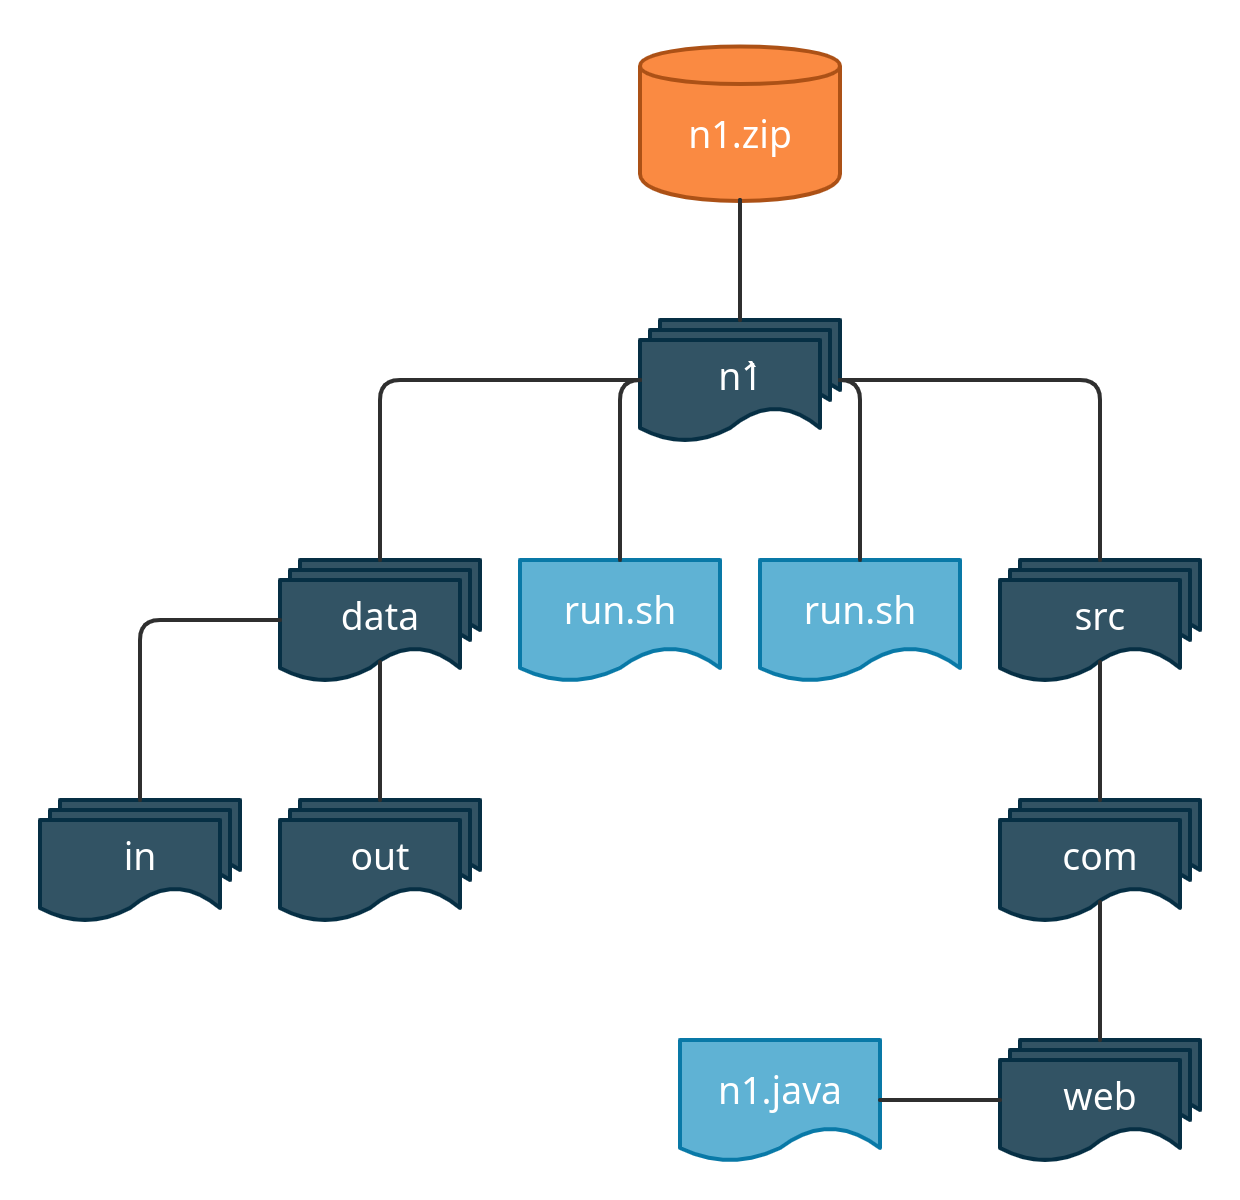
\includegraphics[width=\linewidth]{Figures/zip_example.png}
\caption{Structure of a sample node archive (ZIP)}
\label{fig:nodestructure}
\end{figure}

\subsubsection{Django}

In order to generate the website static files, I utilized the Python library Django. Django is a free and open-source web development framework which enables amazingly powerful out of the box performance and a very good amount of customizability. The website takes advantage of a python virtual environment to manage all of its dependencies. Additionally, to keep the website secure, a ".env" file is used on the web server in order to store sensitive information that a hacker could mine from any requests to and from the server.

\begin{figure}[ht!]
\centering
\begin{tcolorbox}[boxrule=0.5pt,colback=cyan!15!white]
\begin{lstlisting}[basicstyle=\footnotesize, frame=lines]
class AwsAccount(models.Model):
  user = models.ForeignKey(
    		User,
		related_name="aws",
		on_delete=models.CASCADE,
		default=None
  	)
  access_key = EncryptedCharField(
		default=None,
		max_length=255,
		blank=True
	)
  secret_key = EncryptedCharField(
		default=None,
		max_length=255,
		blank=True
	)
  token = EncryptedCharField(
		default=None,
		max_length=255,
		blank=True
	)
class Workflow(models.Model):
  user = models.ForeignKey(
    		User,
		related_name="wf",
		on_delete=models.CASCADE,
		default=None
  	)
  name = models.CharField(
		default=None,
		max_length=255,
		blank=True,
		primary_key=True
	)
  status = models.CharField(
		default=None,
		max_length=255,
		blank=True
	)
class Node(models.Model):
  wf = models.ForeignKey(
    		Workflow,
		related_name="node",
		on_delete=models.CASCADE,
		default=None
  	)
  name = models.CharField(
		default=None,
		max_length=255,
		blank=True,
		primary_key=True
	)
\end{lstlisting}
\end{tcolorbox}
\caption{Django models utilized by the AUI}
\label{fig:djangomodels}
\end{figure}

In order to store information, the website utilizes an sqlite3 database. The database is stored as a local file on the machine and it is where all of the objects and user's information is held. In order to specify the schema of this database, Django utilized what are called models. Models specify a variable name, a data type, and some more metadata about how the data should be treated. This allows users to modify the database schema without the need for advanced knowledge of SQL. In order to ensure security even further, all sensitive information (passwords and AWS credentials) is encrypted prior to going into the database so that, even if somebody were able to view the raw data, it would be extremely unlikely that there would be a data leak. In figure \ref{fig:djangomodels}, the schema for the database can be seen represented as they are in the Django models file. This well-defined data schema is what allows GCC to function as effectively as it does and it is what allows for objects to be associated with different users. As can be observed in figure \ref{fig:djangomodels}, both the "AwsAccount" and "Workflow" class contain a foreign key to the "User" class. This is the feature that facilitates the aforementioned association.

The final main feature of Django that will be discussed in this section is the views feature. In order to facilitate a page on a server, Django uses what are called view functions which can be associated with specific URLs. By implementing a view function, you can control which files are served whenever a specific URL is visited. This feature allows the website to process a request, run code that is needed for that request, and return a response in an incredibly intuitive manner. It is in this way that the web server is able to execute a user's workflow object. When the user clicks on the execute button, they are temporarily redirected to the executing view which calls for the execution using a Python subprocess. Once this subprocess is called and is out of the way, the user is then returned back to the "Execute a Workflow" page where they began. It is for this reason that an execution can be run asynchronously so that a user does not have to be logged into the web page in order for their execution to continue. Views provide even further functionality by serving information with each request. This information is what makes it possible to display workflow objects that are associated with a user as well as serve forms that contain the means to receive information.

\subsubsection{Hosting}

In order to serve the static files generated by the Django source, GCC utilizes an OpenStack instance which is configured with an Apache 2 server. The reason for this is that the instance can be constantly running and serving files, making it available to all at any time of the day. The Apache 2 server is configured to read files from a directory called "gcc\_dep" and it is instructed to use the environment which is available in this directory to ensure that all required packages are being utilized. For an added layer of security, all files on the server are access restricted so only sudo users can access these files. The only way to gain sudo privileges is to connect over ssh and that is restricted to only those who have access to the machine's secret key. This added layer of serves to further enforce strict data security practices.

\subsection{CWFP}

The CWFP (Comprehensive Workflow Planner) is an algorithm, written in java, that intakes a workflow specification file from a user and converts that file into a directed acyclic graph. This graph represents the dependencies between nodes in a workflow. It consists of two main pieces: an XML parser, and a planning method which turns the raw information into the desired directed acyclic graph.

\subsubsection{XML Parser}

The XML parser is the portion of the CWFP that handles the raw input data. When a workflow is set to be executed, the XML parser intakes the path to a specification file, the name of the user who's requesting an execution to take place, and the name of the workflow which is to be executed. In order to perform the parsing procedure, this method utilizes the "org.w3c.dom" and "javax.xml.parsers" libraries which work together to break down an XML file into different objects which can then be analyzed and have the data stripped out of them. Initially, the document is converted into a "NodeList" object using the method "getElementsByTagName('task')". This method reads in the XML data and creates a list of each object labeled "task" that is within the specification file. An example of this is represented in figure \ref{fig:xmlspec} where each element consists of an object with the label "tag". After this list is created, it is iterated over using a for loop and the contents of each object are extracted and stored as string variables within the loop. This information is then placed into a new NodeADT object and that node is added to an ArrayList as well as a HashMap which is used to correlate a node's id to its corresponding NodeADT object. This information is stored locally within the CWFP class and it is not returned to the main method since it is not used there.

\subsubsection{Planner}

\begin{figure}[t!]
\centering
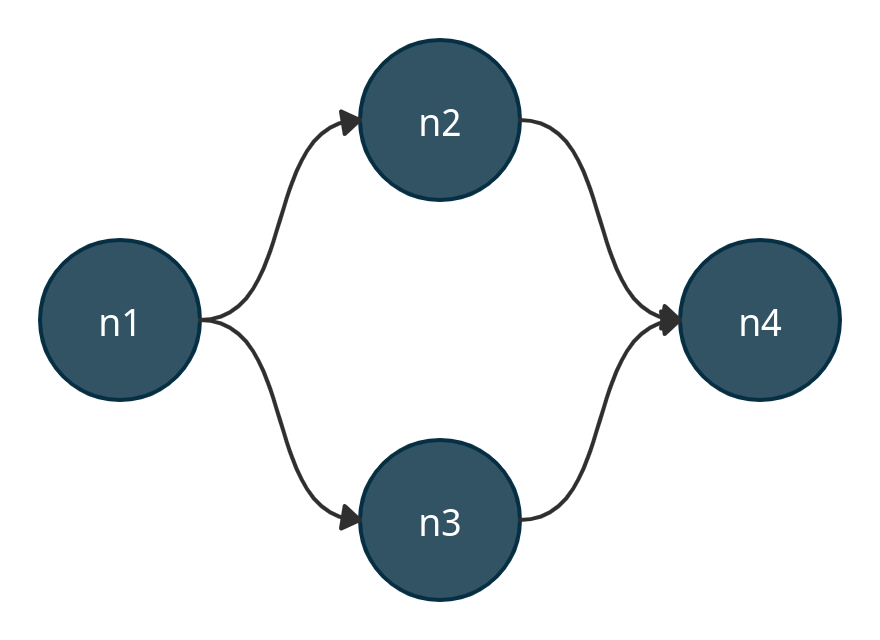
\includegraphics[width=\linewidth]{Figures/dag_example.png}
\caption{Example graph generated by running the workflow in figure \ref{fig:xmlspec} through CWFP}
\label{fig:dagexample}
\end{figure}

As mentioned before, the workflow planner creates a directed acyclic graph data type to represent a workflow object. In order to do this, the planning function utilizes the ArrayList and HashMap that are created by the XML parser. Firstly, two ArrayList objects called "lint" and "compIds" are created, as well as an integer "max" which is initialized to zero. Next, a while loop is created and it runs until it is broken out of using a logical break statement within the loop. Also within this loop, there are two for loops. These for loops are not nested. In the first for loop, all of the nodes in a HashMap "hm" are iterated through. Initially, "hm" is empty so the first for loop does not run on the first iteration of the while loop. If "hm" is populated, "lint" and "compIds" receive the node and node id for each object within "hm" respectively. Once this is done, a logical check happens to see if "lint" is equal to the ArrayList set by the previous section. If this is true, then the while loop is broken out of. If it is false, the second main for loop is invoked. This check is to ensure that when everything is added to the graph that the while loop does not continue to run. If the second main for loop is invoked, meaning the planning has not completed, it iterates through each node in the ArrayList from the XML parser. For each node, there is some validation that occurs to make sure it is valid and exists, and then it is added to the HashMap "hm". This marks the end of an iteration of the outer while loop and, depending on if "hm" is fully populated or not, it will run again. Once outside of this while loop, all levels within "hm" are inserted into a directed acyclic graph and this is returned to the user. Each graph contains a set of nodes, and each node contains a set of edges which allows for an efficient execution once the graph is created. Figure \ref{fig:dagexample} shows the directed acyclic graph that would result from running the workflow specification from figure \ref{fig:xmlspec} through the CWFP. Algorithm \ref{alg:algorithm1} provides a visual representation of the CWFP's approach. In this algorithm, ledger is simply a HashMap linking a node object to it's respective id. Additionally, figure \ref{fig:mapexample} shows a table which represents the mapping that takes place in GCC to execute a workflow. This table shows the mapping for the workflow shown in figure \ref{fig:dagexample}. The table contains a cost element as this is a very important part of workflows. Currently, GCC has the ability to execute workflows using any type of algorithm that it is provided. It was designed in a way to make it more managable and customizable in the future. One algorithm that currently works in GCC is the BHEFT algorithm. This algorithm takes into account execution time and budget constraints to execute workflows in both a time and cost effective manner \cite{verma2015cost}. This allows users greater control over their executions and ensures that their plans stay within a comfortable budget range.

\begin{figure}[t!]
\centering
\begin{center}
\begin{tabular}{|| c | c | c | c ||}
	\hline
	\textbf{Node} & \textbf{Level} & \textbf{Execution Time (hr)} & \textbf{Cost (\$)} \\
	\hline\hline
	n1 & 1 & 10 & 0.072 \\
	\hline
	n2 & 2 & 5 & 0.036 \\
	\hline
	n3 & 2 & 5 & 0.036 \\
	\hline
	n4 & 3 & 2.5 & 0.018 \\
	\hline
\end{tabular}
\end{center}
\caption{Mapping of tasks by the CWFP using the graph in figure \ref{fig:dagexample} as a reference}
\label{fig:mapexample}
\end{figure}

\begin{algorithm}
\footnotesize
\SetKwInOut{Output}{Output}
\SetKwInOut{Input}{Input}
\DontPrintSemicolon
\Input{HashMap$<Integer(K), ArrayList(V)>$ hm}
\Output{DirectedAcyclicGraph$<NodeADT, DefaultEdge>$ pl}
\For {$key \in hm$} {
	$ArrayList<NodeADT> nl \gets hm.get(key)$

	\For {$n \in nl$} {
		$pl.addVertex(n)$

		\If {$n.getDeps() \neq null$} {

			\For {$dep \in n.getDeps()$} {

				$pl.addEdge(ledger.get(dep), n)$
			}
		}
	}
}

\caption{CWFP Algorithm}
\label{alg:algorithm1}
\end{algorithm}

\subsection{Plan Executor}

The WFPE algorithm utilizes both the hashmap and directed acyclic graph created in the previous section in order to begin execution. Within this algorithm, there are a lot of steps taken to ensure that each NodeADT object contains all of its required information. One piece of this information which is the most important is setting the "child" and "parent" node attributes for a node. These two attributes are used extensively during the execution of a specific node so it is very important to have an algorithm which ensures these objects are in place and correct. Additionally, the WFPE algorithm handles the execution of the overall workflow plan that is provided by the CWFP algorithm. To do so, the WFPE utilizes yet another for loop and while loop combination. The while loop is constantly running until a break condition is met within it, while the for loop iterates over the HashMap for each level in a workflow.. The break condition for the while loop is very simple and it can be stated as follows: if the total number of nodes that are done executing in a level is equal to the total number of nodes in that level, then break. In order to count the number of total nodes that are completed, the WFPE utilizes data from the node objects themselves. Each node object contains an object of the "ExecInfo" class which contains all of the execution information for a specific node. While in the while loop, the WFPE checks for each node in a specific level of the workflow to see if a boolean value which represents execution status is true or false. If the variable is true, then the variable representing the total number of completed nodes is incremented by one. Finally, once this number is equal to the number of nodes in the level, the for loop runs again for another level within the workflow. This combination of tasks allows for each level to be executed in the correct order. In order to begin the execution of a node itself, the WFPE utilizes a multi-threaded approach which calls the NEF for each node in a level simultaneously. This dramatically reduces the execution time as doing this in a linear fashion would require one node in the same level of another node to wait for it's peer to finish until it could begin. In order to preserve computing resources, a "Thread.sleep(500)" is included in the while loop so checks for execution status only happen every half a second. This is realistic because on the scale of large computations, a latency of half of a second is negligible and the price of upkeep of an instance for this time period is extremely small, especially when it is not transferring data or utilizing any computing resources. Algorithm \ref{alg:algorithm2} shows a visual representation of the execution portion of the WFPE algorithm.

\subsection{NEF}

Finally, The NEF algorithm is the algorithm that executes a payload on a node when that node is designated by the WFPE to be executed. This algorithm consists of 5 main stages which work together and communicate with other nodes in order to provide a successful execution environment. The first of these stages is the provisioning stage. When in the provisioning stage, the NEF algorithm checks to see if an instance for a node has been initialized. When this node is first being called, this will be false by default. If the instance is not initialized, the NEF algorithm initializes a new instance using the AWS API. For testing reasons and the scope of this project, all resources are set to the "t2.micro" size and the image is of the Ubuntu 20.04 distribution. Once the initialization has begun, the NEF algorithm waits until the instance status code returned is equal to 16, which ensures that the instance is available for SSH connections on port 22. Once the instance is provisioned, the NEF stops waiting and moves on to step 2. Now that SSH connections can be made to the instance associated with a node, step 2 consists of transferring the nodes payload to the instance, installing java and unzip using the apt package repository, and unzipping the payload to get it ready for execution. This step is pivotal as it is what enables a proper execution environment for a node. Once the node payload is extracted and it's basic file system remains, then a node can have it's dependencies transferred to it. Here marks step 3. Step 3 only takes place if a node has one or more dependencies. If this is not true, then this step is skipped. If it is true, then for each node which the current node depends on, the files in the "data/out" folders of that node's virtual machine are transferred to the "data/in" folder of the current node's virtual machine. This ensures that each node has all of the proper data that it needs in order to execute properly. Upon the successful completion or surpassing of step 3, step 4 begins. In step 4, the node's payload is compiled and executed using the scripts which are provided by the user. This step is quite simple yet it relies heavily on steps 1-3 to be done correctly. After step 4, step 5 begins and this is where instances are either terminated or not. If a node has children which depend on its results in order to function, the node will be left dormant until it's files are required. If the node does not have any children, then it's virtual machine can safely be terminated. Additionally, for any node with no children, the contents of the "data/out" folder on that node's virtual machine are downloaded to the execution server to be later shown to the user. It is important to note that, throughout the process of the execution, the NEF algorithm continually collects logs for each command that is executed on a virtual machine. For each node, these logs are printed to a text file with the nodes id followed by a "\_logs.txt" fragment which allows users to view what is happening on the virtual machines for each node and possibly debug execution errors.

\begin{algorithm}
\footnotesize
\SetKwInOut{Output}{Output}
\SetKwInOut{Input}{Input}
\DontPrintSemicolon
\SetKwBlock{DoParallel}{do in parallel}{end}
\Input{ArrayList$<NodeADT>$ nl}
\Output{Results from executed workflow}

\For {$nl \in hm.values()$} {

	$done\_ct \gets 0$

	\For {$n \in nl$} {

		\DoParallel {
			$executor.execute(n)$
		}
	}
	\While {$true$} {

		\If {$done\_ct == nl.size()$} {

			$break$
		} \Else {

			$done\_ct \gets 0$

			\For {$n \in nl$} {

				\If {$n.ei.getExecStatus() == true$} {

					$done\_ct \gets done\_ct + 1$
				}
			}
		}
	}
}
% \DoParallel{
%
% }

\caption{WFPE Algorithm}
\label{alg:algorithm2}
\end{algorithm}

%------------------------------------------------

\section{Experimental Results}
\label{sec:expresults}

In this section, some preliminary experimental results will be discussed. These preliminary tests serve as a proof of concept as well as a performance analysis for the GCC framework as a whole. All tests were performed on the same machine under the same network environments. Each execution was performed just as the last to ensure consistent results.

The first round of testing that occurred was comparing the number of nodes in a workflow to that workflows makespan. This testing occurred with workflows of sizes 5, 10, 15, and 20. Due to a restriction that Amazon places on the maximum number of instances allowed in a certain region for a user, 20 was the largest test case that could be produced. In each workflow that was tested for the sake of this comparison, there were 3 levels present. Both levels 1 and 3 consisted of a single node and level 2 consisted of 3, 8, 12, and 18 nodes respectively. This resembles a distributed approach in which data is split in the first node, analyzed in all nodes on level 2, and finally re-compiled in the final node. In order to ensure consistency, an arbitrary "Thread.sleep(10000)" was the payload for each node and a 5 MB file was transferred from each node to it's dependents (if it had any). The results of this execution are shown in figure \ref{fig:tr1}. As can be observed, there is a gradual increase on the x axis with respect to the number of nodes in a workflow, however this is not linear. The $R^2$ value of the trendline for these data points was 0.703 meaning that the trendline was not exactly linear. The reason for this is the multi threaded approach that is taken when executing nodes on a given level. This approach provides a runtime which is theoretically capped at how many levels are in a workflow. As an unexpected result, however, it can be observed that there is a clear positive, non-zero slope to the trendline meaning that increasing nodes on a level does increase the execution time of the workflow. This result was surprising but the explanation lies in step 3 of the NEF algorithm. When files are transferred to a node from one of its parent nodes, this transfer happens on a single thread and utilizes a linear approach. When more nodes are added to a workflow, more transfers must be made to the final node on level 3. It is for this reason that a non-zero increase in makespan can be observed when the number of nodes in a workflow of 3 levels, where the final level depends on all previous nodes, is increased.

\begin{figure}[t]
\centering
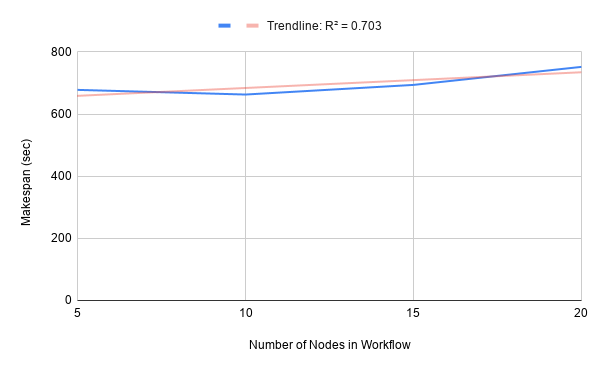
\includegraphics[width=\linewidth]{Figures/makespan_vs_nodecount.png}
\caption{Makespan Vs. Number of Nodes in Workflow}
\label{fig:tr1}
\end{figure}

\begin{figure}[t]
\centering
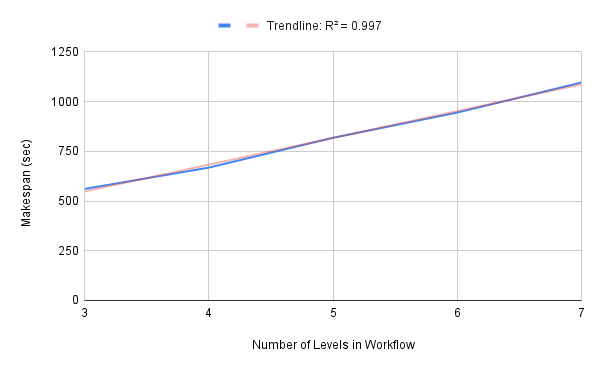
\includegraphics[width=\linewidth]{Figures/makespan_vs_levelcount.png}
\caption{Makespan Vs. Number of Levels in Workflow}
\label{fig:tr2}
\end{figure}

\begin{figure}[t]
\centering
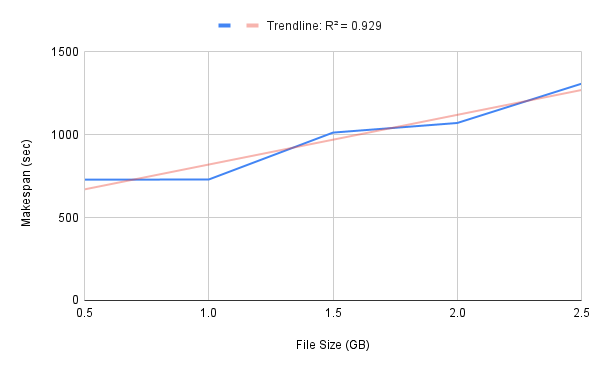
\includegraphics[width=\linewidth]{Figures/makespan_vs_filesize.png}
\caption{Makespan Vs. File Size}
\label{fig:tr3}
\end{figure}

For the next test that was conducted, the number of levels in a workflow were increased and a makespan measurement was taken for each test case. The number of levels tested for each iteration was 3, 4, 5, 6, and 7 respectively. For the purposes of this test, all levels only contained one node with the same arbitrary wait time and 5 mb file transfer as before. This was done to ensure consistency between tests. As can be observed in figure \ref{fig:tr2}, the regression coefficient for the test was almost exactly 1 (0.997). This means that there is a strong direct correlation between the number of levels in a workflow and the total makespan. For each test with different level counts, the average increase to the makespan was 133.75 seconds. This result was not particularly surprising as there is no current methodology in the GCC framework for executing nodes on levels that are dependent on previous levels before those levels are done executing. This test shows the linearity of adding levels to a workflow and it is a helpful piece of knowledge to have especially taking into account that makespan directly correlates to the amount of money a user will spend when executing a workflow.

The final test that was conducted during this preliminary experimentation phase was the effect that file size has on the makespan of a workflow. In order to test this, workflows which each contained four nodes and 3 levels, much like that shown in figure \ref{fig:dagexample}, were executed. The payloads in the workflow were different for each level. For testing purposes, the workflow executed a diamond pattern character counting procedure in which the node on the first level would split an input file into two separate parts and send these parts to the two nodes located on the next level. These two nodes then counted the characters in the file which they received and, once both were completed, the output from them was sent to the final node which simply aggregated the data into one final result. It is important to note that the main time bottleneck in this workflow resides within the first two levels. The file sizes that were tested were 0.5, 1, 1.5, 2, and 2.5 gigabytes respectively. The results of the experiment are shown in figure \ref{fig:tr3}, and a fairly constant upward trend can be observed. This trend has a regression coefficient of 0.929 meaning it is sufficiently linear. As with the previous experiment, this would indicate a strong positive correlation between file size and makespan. One possible trend that can also be observed in \ref{fig:tr3} is the sort of step-up progression of the data points. When going from a file with a gigabyte value that is an integer to a file whose gigabyte value is in between integers, there is a visible increase in the makespan which is more significant than that of the transition back to an integer value. When developing these tests, one thing to note is that a large majority of the makespan consisted of the NEF transferring a nodes payload which contained rather large files. Combining this knowledge with that learned from experiment two, it is safe to say that the worst case run time of the GCC framework can be achieved by executing a workflow with a high data overhead and multiple levels. It is important that these limitations and worst-case scenarios are understood in order to improve upon the methods in the future.

%------------------------------------------------

\section{Related Work}
\label{sec:relatedwork}

As the problem of task scheduling in computer science is increasingly important, there has been copious amounts of research surrounding the topic in the recent past. In this section, nine articles which pertain to GCC will be discussed along with their methods and results. The first article to analyze is entitled “Symbiotic Organism Search optimization based task scheduling in cloud computing environment

”. In this article, Abdullahi et al. discuss a task scheduling algorithm which relies on a symbiotic organism search optimization. This type of optimization is named according to the similarity it shares with symbiotic organisms in nature; those who share a beneficial relationship between each other. The findings of this article were a search optimization framework that functions better than particle swarm optimization when searches get larger \cite{abdullahi2016symbiotic}. This is a significant finding as PSO is one of the most popular frameworks used in cloud computing today.

In “Enhanced particle swarm optimization for task scheduling in cloud computing environments”, Awad et al. propose LBMPSO which aims to combine PSO with load based management in order to provide reliability and load balancing. The findings of this article were that in cloud execution environments, LBMPSO was able to successfully provide a load-balanced reliable framework which did not significantly increase the total makespan of a workflow \cite{awad2015enhanced}. This is extremely important because it allows for more reliable executions which run very efficiently.

Another popular work scheduling algorithm is a genetic algorithm. Genetic algorithms are algorithms that function just as organisms do in the theory of evolution. For each lifecycle, the algorithms adapt and the weaker generations die off. This leads to the ability to create highly optimized algorithms based on training and testing. In “The Study of Genetic Algorithm-based Task Scheduling for Cloud Computing”, Jang et al. explore an alternative task scheduling algorithm which takes this approach \cite{jang2012study}. What the authors found was that genetic algorithms provide large increases in efficiency when compared to linear or round-robin based algorithms which performt the same basic task. Similar findings were documented in “An efficient approach to genetic algorithms for task scheduling in cloud computing environment” as well \cite{kaur2012efficient}. Genetic algorithms of the past stand as the basis of where the field currently resides.

As well as the two most popular task scheduling algorithm frameworks, much work has been done developing other frameworks as well. Such work can be observed in “Task scheduling for cloud computing using multi-objective hybrid bacteria foraging algorithm” in which the authors explore and employ an algorithmic representation of bacterial foraging which is designed to optimize the efficiency of task scheduling. As a testament to the prevalence of genetic algorithms in the field, the authors also utilized some genetic methods in their final proposed result. The findings of the article were that significant makespan, cost, and overall time optimizations were able to be achieved in the proposed framework \cite{srichandan2018task}. These results are very exciting and bring a lot of possibility for the future of the field as they show just one of the ways that existing genetic frameworks can be improved upon.

%------------------------------------------------

\section{Conclusion and Future Work}
\label{sec:conclusion}

Gator Computational Cloud is a technology that was made for the purpose of providing accessible, usable, and efficient workflow execution services in a lightweight delivery method using a web application. In this paper, we propose this tool as a solution to the ever changing task-scheduling problem. The tool utilized a multi-threaded approach to provision instances and execute nodes in a way that is specified by the user rather than the tool itself. This allows for amazing levels of customization and usability while also upholding a low barrier to entry as the design of a workflow specification is not overly complicated and can be taught with few instructions. In its current state, the tool is capable of handling any type of workflow that is provided to it. Depending on how many levels or nodes are in the workflow, as well as the size of the data that is being processed, execution times may vary. In the future, the refinement and expansion of this tool is very feasible and could possibly provide some real use cases outside of academia. In order for this to be the case, all code would need to be assessed and rethought if needed. This will allow for more consistent and better performance which would make the tool a lot more practical. One specific area of improvement which would greatly increase the practicality of the tool is making file transfers to a child node from parent nodes asynchronous as the level-based execution is now. In the end, the ever-increasing amount of data in this world makes GCC more and more relevant as each day passes and, while still maintaining the same goal of providing accessible and usable utility to a user, there are many directions that GCC can go in the future to improve.

%----------------------------------------------------------------------------------------
%	REFERENCE LIST
%----------------------------------------------------------------------------------------

\phantomsection
\bibliographystyle{acm}
\bibliography{refs.bib}

%----------------------------------------------------------------------------------------

\end{document}
